% !TEX root = ../main.tex
\chapter{Whole-System Emulation}
\label{chap:3}

Virtualization is the process of abstracting the hardware components of a system in order to make them available to software in a virtual form.
The word virtualization today is used to identify both generic virtualization and whole-system emulation, however, as it will become clear later, this two systems are completely different and applications in the real word.

First of all virtualization iself can be divided in 3 categories: modern processors have built in support for virtualization meaning that the system is able to execute virtual machines, on the physical CPU in complete isolation, this is called \textbf{hardware assisted virtualization}. \textbf{Paravirtualization} and \textbf{full virtualization} are older methods that requires either the modification of the guest system or partial emulation of the CPU. In particular in \textbf{Paravirtualization} the hypervisor provides an API and the guest OS makes calls to that API. \textbf{Full virtualization} relies on binary translation to trap and virtualize the execution of certain non-virtualizable instructions, this approach requires that critical instructions are discovered and replaced with traps that will implement such instructions in software.

A typical use of virtualization would be to share resources of a single system between multiple users or to have multiple Operating Systems on the same machine. This is done by providing a thin layer of abstraction on top of the physical hardware in order for it to be shared, concurrently among multiple virtual systems. The limit of this virtualization is that there will always be a 1 to 1 correspondence between virtual and physical hardware. Meaning that, on top of a defined architecture, the virtual processors can be only of the same architecture as the virtual one: on top of a physical 64 bit processor the virtual one will be a 64 bit processor as well. Such system provides different advantages: first of all the abstraction of the CPU can be accomplished with a very low overhead as the instructions for the virtual CPU can be run directly on the physical one moreover, modern CPUs have some very specific mechanism in order to have an efficient virtualization.

Whole-System emulation is a completely different method that allows to run different architectures on top of a single one. As a matter of fact the CPU, and possibly other devices, are implemented in software introducing an intermediate layer that allows a program compiled for a specific architectures to be run on different ones. It is clear that this method introduces a much higher overhead compared to the previous one as, in order to translate instructions from an architecture into another, there is the need for a middleware that performs such conversion at run time.

The Operating System on top of which the virtualization software runs is called Host OS while the Operating System that run inside each virtual machine is called Guest OS. The glue layer between physical and virtual hardware is called hypervisor or Virtual Machine Manager, this term applies both to hardware assisted virtualization and whole-system emulation as it will be explained in the following sections.

One of the most famous tools that provides both virtualization and whole-system emulation modes is QEMU (Quick Emulator). In emulation mode it uses an intermediate language called TCG to translate instructions between two architectures at run time and is often referred to as QEMU-TCG. In virtualization mode it leverages kernel drivers such as KVM (Kernel-based Virtual Machine) in order to create proper virtual machines in the same way as VirtualBox or VMWare. Another feature of QEMU that contributed to its popularity in the security research field is that it is Open Source and this allows to perform deep modifications into the source code in order to add or expand its functionalities.

\section{A bit of background: the Hypervisor}

At the core of the virtualization process there is the Hypervisor. The hypervisor is a piece of code whose definition blends with the one of operating system. Hypervisors are also commonly referred to as Virtual Machine Managers (VMM) in fact they take care of all the tasks related to the management of resources and integration between physical and virtual machine, effectively creating an interface between the two.

Virtualization requirements have been defined in \cite{virtreq} and proposes a set of properties that Virtual Machine Monitor should have:

\begin{itemize}
    \item \textbf{Equivalence / Fidelity:} A program running under the VMM should exhibit a behavior essentially identical to that demonstrated when running on an equivalent machine directly.
    \item \textbf{Resource control / Safety:} The VMM must be in complete control of the virtualized resources.
    \item \textbf{Efficiency / Performance:} A statistically dominant fraction of machine instructions must be executed without VMM intervention.
\end{itemize}

Although in the years such properties have been revised and nowadays for a VMM to be considered as such it is sufficient that it verifies the first two. 

As described in\cite{os} there are 3 different types of hypervisors: \textbf{Type 0}, \textbf{Type 1} and \textbf{Type 2}. 

Modern processors have virtualization support built in the hardware meaning that the processor offers an additional layer on top of which the VMM can operate. This allows to have hardware hypervisors, often referred as \textbf{Type 0}. This piece of code runs directly on the hardware and takes care of allocating the right amount of resources and handle hardware-software interactions. This method is really close to running a proper operating system directly on the physical machine as each virtual machine created by a\textbf{Type 0} Hypervisor effective runs, in turn, on the physical CPU. For this reason each VM created in this way can be a different kind of VMM itself. This type of hypervisor are highly specialized firmwares and for this reason also uncommon to be found in the wild, as a matter of fact they are often found in very specific devices such as mainframes. 

In addition to this all modern CPU implements a form of Hardware Assisted Virtualization, called VT-x for Intel and AMD-V for AMD. Hardware virtualization allows for better performance and easy maintaining of the virtualization software by expanding the CPU instruction set with some dedicated instructions. 

A graphical representation of the differences between the other two types of hypervisors can be found in Figure \ref{fig:hip}.

\begin{figure}[htp]
\centering
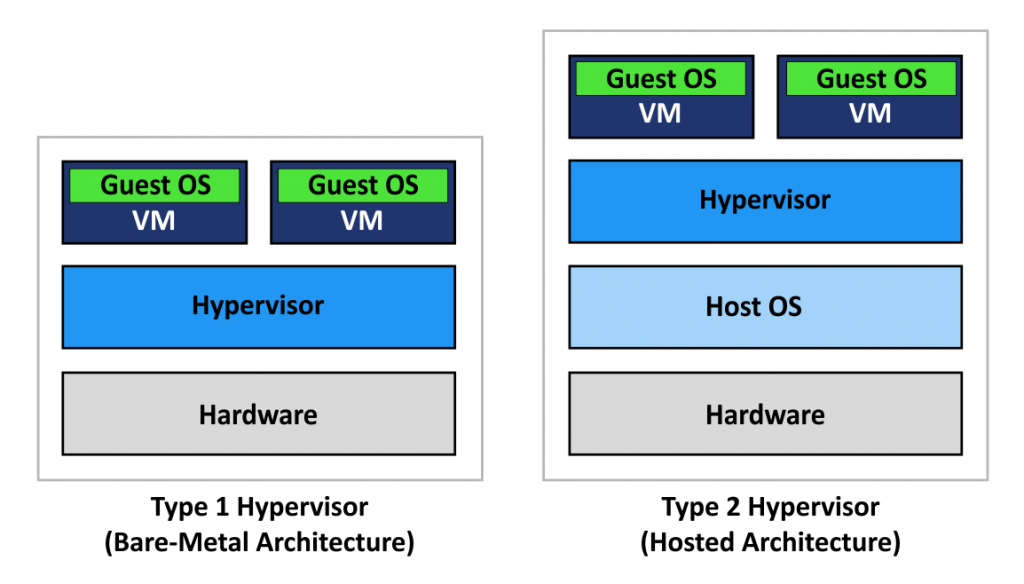
\includegraphics[width=\linewidth]{images/hip.png}
\caption{Hypervisors types \newline \url{https://netseedblog.com/security/virtualization-forensics-part-1/}}
\label{fig:hip}
\end{figure}



\subsection{Type 1 or Bare-Metal}

The \textbf{Type 1} or "Bare Metal" hypervisor is a a sort of specialized operating system that is dedicated only to the management of virtual machines. This is very commonly found on servers, particularly in data-centers where it is necessary to have high efficiency on single servers. For this reason VMs that run on this type of hypervisor can achieve very high performances due to the fact that, similarly to \textbf{Type 0}, they allow guest VMs to run directly on the hardware. Examples of this kind of hypervisor are VMWare ESX and Xen.

Moreover even non specialized operating systems such as Linux, Windows and MacOS have support for virtualization and can act as \textbf{Type 1} hypervisors. As they are not dedicated VMMs they provide fewer control and customization over the virtualized environment and they have slightly lower performances as treat the virtual machine like every other process. However, virtual machines that run on this kind of hypervisor are still efficient as they will be granted direct access to system resources. 

\subsection{Type 2 or hosted}

The \textbf{Type 2 }hypervisor is a dedicated piece of software which provides another layer of abstraction as it runs on top of an existing operating system. Virtual Machines running on top of this hypervisor will not have access to the real physical hardware and instead they will access an emulated and standardized architecture. In this way the user can have more control on the resources and the virtualized environment, trading in some performances. 

It must be noted that nowadays this two types of hypervisors can, sometimes, blend together. For example Linux KVM (Kernel Based Virtual Machine) is a kernel module available in modern Linux distributions that transforms the operating system into a \textbf{Type 1} hypervisor while still retaining all the other OS functionalities.


\section{Emulation}

Virtualization and emulation bring some benefits mainly in terms of:
\begin{itemize}
    \item \textbf{Efficiency} as multiple virtual machines can be run on a single physical machine optimizing the usage of resources.
    \item \textbf{Cost reduction} derived directly form the above one, by more efficiently utilizing a single machine it is possible to "do more with less".
    \item \textbf{Compatibility} as different Operating Systems can run on a single host OS this allows to run, compile or test different applications on top of a single environment almost closing the gap between the various architectures.
    \item \textbf{Easier testing} as different architectures can be emulated on top of a single machine this allows to develop programs for different architectures bypassing some unnecessary steps, for example an application for a phone can be complied and tested on a normal laptop and then pushed to the phone only when the final version is ready.
    \item \textbf{Security} perhaps the most important fact, as virtual machines are all isolated between them and between the guest OS they can be managed in a better way. Moreover the ability to take snapshot of a certain state and then revert the machine back to it makes it more resilient to attacks, avoids potential data loss and makes it more resilient to software faults. 
\end{itemize}

As discussed above there are different approaches that can be taken to virtualize an environment. One of the most interesting techniques is \textbf{Emulation}. 

This technique takes virtualization even further as the main component of a system, the CPU, needs to be completely re-implemented in software. This means that while in pure virtualization there was somehow a correspondence and an interaction between the guest system and the real system, i.e. instructions generated for the virtual CPU could be run \underline{directly} on the physical one. On the emulated environment, instead, there is the need to have a different, and more complex, type of virtual CPU. This virtual processor perform the translation between the instructions coming from the guest system into instructions that can be executed on the host system.

This poses different challenges on the implementation side: 

the translation must be quick and efficient to introduce the lowest possible overhead.

In order to support the maximum number of virtual and physical CPUs the system should be easily expandable meaning that an intermediate structure must be introduced to provide and architecture agnostic instruction set.

Every instruction must be correctly emulated and translated or handled in order to provide a fully working emulated CPU, this has also some advantages as some instructions can be handled directly via software without the need of converting them.

\section{Virtual Machines}

With the term Virtual Machine we usually refer to \textbf{Type 2} hypervisors.

There are available different solutions to create virtual machines, both open source and commercial ones. Between the open source solutions \textbf{Virtual Box} and \textbf{QEMU} are the most common while on the commercial side \textbf{VMWare} and \textbf{Paralles} are the main players. 

There are many things that must be coordinated under the hood in order to successfully trick the Guest OS into believing that it is running on a physical machine and has dedicated resources. Some peculiar aspects are memory management and CPU scheduling.

On the memory management side there is a high pressure on the real memory which will be used by the Host OS, Guest OS and by the VMM itself. There is therefore a need for an efficient management of the RAM:

\textit{"Before memory optimization can occur, the VMM must establish how much real memory each guest should use. To do that, the VMM first evaluates each guest’s maximum memory size. General-purpose operating systems do not expect the amount of memory in the system to change, so VMMs must maintain the illusion that the guest has that amount of memory. Next, the VMM computes a target real-memory allocation for each guest based on the configured memory for that guest and other factors, such as over commitment and system load"}\cite{os}

The physical CPU will be under stress as well as it will be shared between Guest OS, Host OS and VMM. This latter software has access to the real hardware and can therefore steal CPU cycles from the Guest OSs to schedule its tasks for VM Management.
\textit{"More difficult is the case of over commitment, in which the guests are configured for more CPUs than exist in the system. Here, a VMM can use standard scheduling algorithms to make progress on each thread but can also add a fairness aspect to those algorithms"}\cite{os}

I/O is another interesting aspect of the virtualization that must be taken into account, a VMM must create proper virtual devices such as Network Bridges in order to allow each machine to connect to the network. There are moreover devices such as webcams or USB storage which cannot be accessed concurrently therefore there is no alternative if not to allow a single machine at the time to use them.


\section{QEMU}

\todo{briefly mention bochs as it will come back duriing paranoid tests}
QEMU is a powerful open source virtualization software which can operate in two modes: 

\textbf{User-Mode emulation} which allows QEMU to run programs compiled for a CPU on another CPU.

This working mode differs from whole-system emulation as the only device that is emulated here is the CPU moreover, such CPU is used to run only the user space code and in particular the code of the program to be run. The different signals generated by that program are then captured and converted in native ones which can be executed on the host machine. A visual representation of this mode can be seen in Figure \ref{fig:quser}.

\begin{figure}[htp]
\centering
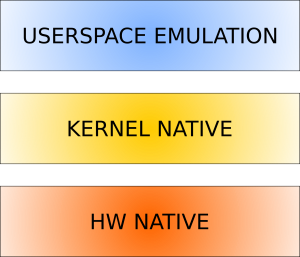
\includegraphics[width=7cm]{images/qemu-user.png}
\caption{QEMU user mode emulation\cite{quser}}
\label{fig:quser}
\end{figure}

In particular the following 3 features are handled by QEMU when running in user mode:

\begin{itemize}
    \item \textbf{System Calls:} are converted to fix endianness and 32/64-bit mismatches between hosts and targets. I/O commands is be converted as well.
    \item \textbf{Signals:} are redirected from the host to the running program, signals are also generated from exceptions happening in the virtual CPU.
    \item \textbf{Threads:} the \lstinline{clone} system call is emulated and a real thread is created on the host. Each of this threads will have a separate virtual CPU.
\end{itemize}

In this way a big part of the emulation process is avoided and the execution is much faster than in Whole-System Emulation mode. However, in order for QEMU to correctly run the executable it needs to process also all the related dynamic linked libraries. 

Due to this high flexibility and the ability to run virtually any type of executable extracted from a system on an arbitrary User-Mode emulation is widely used in software testing and in fuzz testing, for example in \cite{QASan-SecDev20} QEMU User-Mode has been used for black-box fuzzing of arbitrary binaries.

\textbf{Full System Emulation} where QEMU fully emulates the entire architecture and acts as a proper \textbf{Type 2} hypervisor allowing to create proper virtual machines. In this operating mode QEMU can also be used for virtualization meaning that it can take advantage of KVM or hardware assisted virtualization to run virtual machines at Kernel level and achieve near native performances. 

In this mode QEMU emulates not only the CPU but also any other I/O device. An interesting approach is the one taken with network cards, the standard behaviour is to create a virtual tapN interface on the host system which can be configured as any other interface in the system. However if no \lstinline{-net} option is specified QEMU uses a user mode network stack that can be seen in Figure \ref{fig:qemunet}. This is particularly interesting as by exposing the SMB server 
QEMU facilitates the sharing of files between the host and the virtual machine and it also gives a high level of control to the user by letting him manage the other two devices (DNS and Firewall/DHCP).

\begin{figure}[htp]
\centering
\begin{lstlisting}
guest (10.0.2.15)  <------>  Firewall/DHCP server <-----> Internet
                      |          (10.0.2.2)
                      |
                      ---->  DNS server (10.0.2.3)
                      |
                      ---->  SMB server (10.0.2.4)
\end{lstlisting}
\caption{QEMU network stack}
\label{fig:qemunet}
\end{figure}

Another important component of QEMU is the Monitor, this can be used to interact with the machine while it is running. In particular it can be used to freeze/unfreeze the machine or save/restore its state from disk. Moreover, it allows to inspect the Virtual Machine without an external debugger.

The Full System Emulation mode is particularly interesting in the field of Security Applications, as a matter of fact having a fully emulated system allows a great control over the internal structures. Such control allows for the implementation of complex analysis techniques which requires introspection and/or manipulation of a running system and that would be hard to implement otherwise. Moreover the ability to have an isolated environment in which a malware can be safely run allowed for the development of malware analysis sadboxes built on top of this QEMU mode. 

In order to perform full system emulation QEMU uses an intermediate language called TCG, this will be analyzed in details in the following section as it is the most important part of the emulator.


\subsection{TCG: Tiny Code Generator}

In order to provide support for a wide range of CPUs QEMU leverages Just In Time (JIT) compilation between assembly instructions. This is accomplished with the use of an intermediate code generator called TCG (Tiny Code Generator). This piece of software takes care of translating instruction for the emulated CPU into intermediate instruction, TCG ops, which are then translated into instruction for the real underlying CPU.

By posing this middle layer QEMU allows to seamlessly support different CPU architectures both for emulation and to run on. Such intermediate layer has essentially two sides:

\begin{itemize}
    \item \textbf{Backend} is the TCG part that is facing the physical CPU. It is responsible of translating architecture agnostic instructions, also called TCG ops, into ones for the real machine.
    \item \textbf{Frontend} is the TCG part facing the virtual CPU. It is in responsible of translating virtual instructions into TCG ops.
\end{itemize} 

There as this is a quite complex system QEMU puts in place some optimizations in order to speed up execution and maintain portability. The most notable ones, taken from \cite{translatorinternals}, are:

\begin{itemize}
    \item \textbf{CPU state optimisations:} the internal state of the CPU is saved in a Translation Block (TB), the translation phase considers that some state information of the virtual CPU cannot change in it. If the state changes a new TB will be generated and the previous TB will not be used until the state matches again the one recorded in it.
    
    \item \textbf{Direct block chaining:} each time a Basic Block is translated it is added to the a TGC cache. In this way if the Program Counter points to a TB that has already been translated QEMU will skip the translation phase and, instead, jump directly to the next TB. This is usually achieved with the use of an indirect jump. On some host architectures (such as x86 or PowerPC), the \lstinline{JMP} opcode is directly patched so that the block chaining has no overhead.
    
    In this process the TCG cache plays a particularly important role as it holds all the basic blocks that have already been translated, once this cache is full the approach taken by QEMU is to flush the entire cache instead of implementing a scheduling algorithm.
    
    \item \textbf{Self-modifying code and translated code invalidation:} the TCG cache will not work in case of self modifying code as QEMU will continue to execute the code that has been already generated on a previous translation. To overcome this problem User-Mode emulation marks a host page as write-protected (if is not already read-only) every time translated code is generated for a basic block. In this way if the program access that page in write mode a violation signal is raised by the host OS. QEMU then invalidates all the previous Translation Blocks for that page and enables write accesses. For system emulation, write protection is achieved through the software MMU.
    
    
    \item \textbf{MMU emulation:} as mentioned before QEMU implements a software MMU in Full System Emulation mode. In this way the MMU virtual to physical address translation is done at every memory access.

    QEMU uses an address translation cache to speed up the translation. In order to avoid flushing the translated code each time the MMU mappings change, all caches in QEMU are physically indexed. This means that each basic block is indexed with its physical address.

    In order to avoid invalidating the basic block chain when MMU mappings change, chaining is only performed when the destination of the jump shares a page with the basic block that is performing the jump.

    The MMU can also distinguish RAM and ROM memory areas from MMIO memory areas. Access is faster for RAM and ROM because the translation cache also hosts the offset between guest address and host memory. Accessing MMIO memory areas instead calls out to C code for device emulation. Finally, the MMU helps tracking dirty pages and pages pointed to by translation blocks.

\end{itemize}

TCG uses a mechanism similar to the one implemented by compilers like GCC where a function prologue and epilogue, which are the small pieces of code used to save and restore the context when entering or exiting functions, are added a compilation time. This same mechanism is used when QEMU calls the different Translation Blocks as it can be seen in Figure \ref{fig:qemutbc}.  

\begin{figure}[htp]
\centering
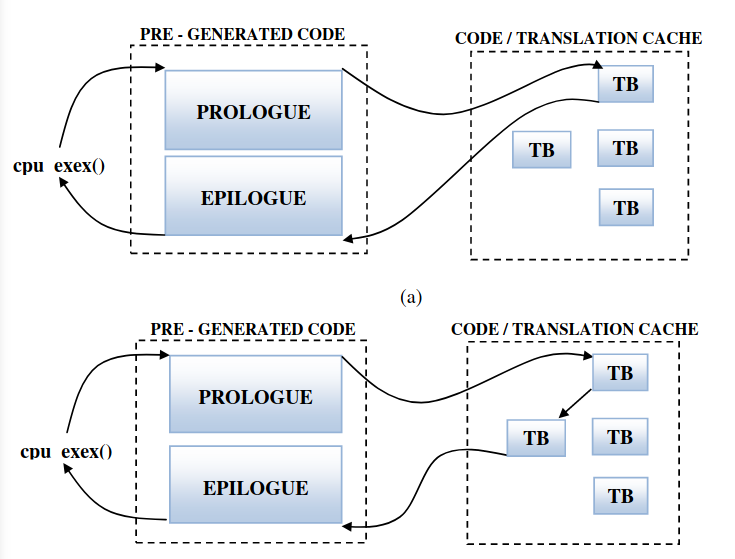
\includegraphics[width=\linewidth]{images/qemutbc.png}
\caption{QEMU translation block(a) and translation block chaining (b)\newline\url{https://lists.gnu.org/archive/html/qemu-devel/2011-04/pdfhC5rVdz7U8.pdf}}
\label{fig:qemutbc}
\end{figure}

The precise flowchart of how instructions are translated between architectures can be seen in Figure \ref{fig:qemuflow}.

\begin{figure}[htp]
\centering
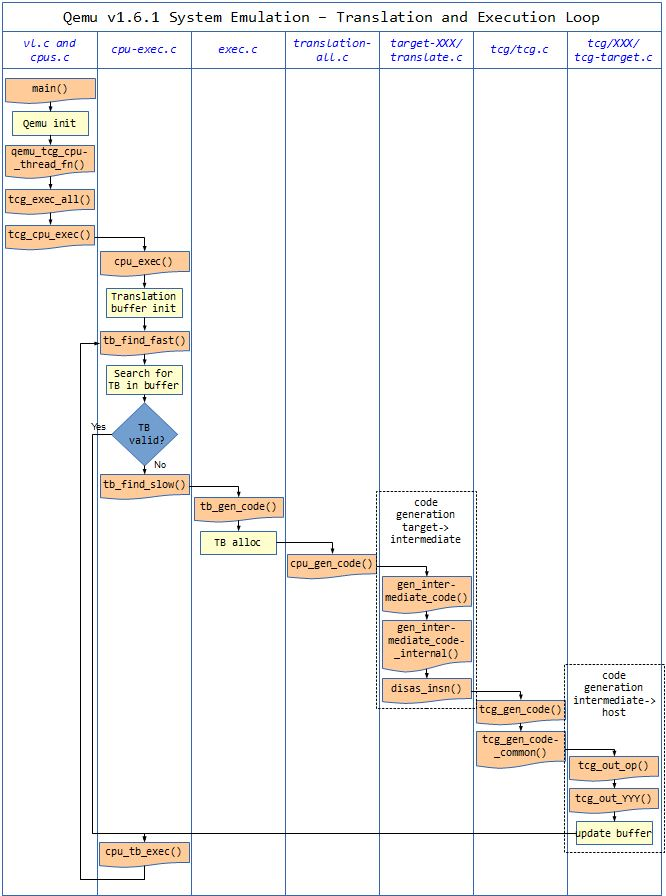
\includegraphics[width=\linewidth]{images/qemutcg.jpg}
\caption{Flow of instruction in QEMU Full System Emulation}
\label{fig:qemuflow}
\end{figure}

For example a typical QEMU execution when an arm binary is run on a x86 CPU is as follows: 
\begin{enumerate}
    \item Instructions from the arm compiled binary are executed on the virtual CPU.
    \item TCG frontend takes care of translating the above instructions into an intermediate language. 
    \item TCG backend trakes care of translating the intermediate instructions into instructions for the real CPU. 
    \item QEMU executes the resulting instructions on the physical CPU. 
\end{enumerate}
